%!TEX root = ../Thesis.tex
\chapter{An Appendix}

%!TEX root = ../Thesis.tex
\section{Draft: \textit{Learning the structure of random forest models in QSAR modelling: Predicting molecular Solubility}}
\label{article:solubility}

This draft has been prepared, however not finished. The draft describes how the solubility prediction model was trained and how to visualize the model structure with forestFloor.

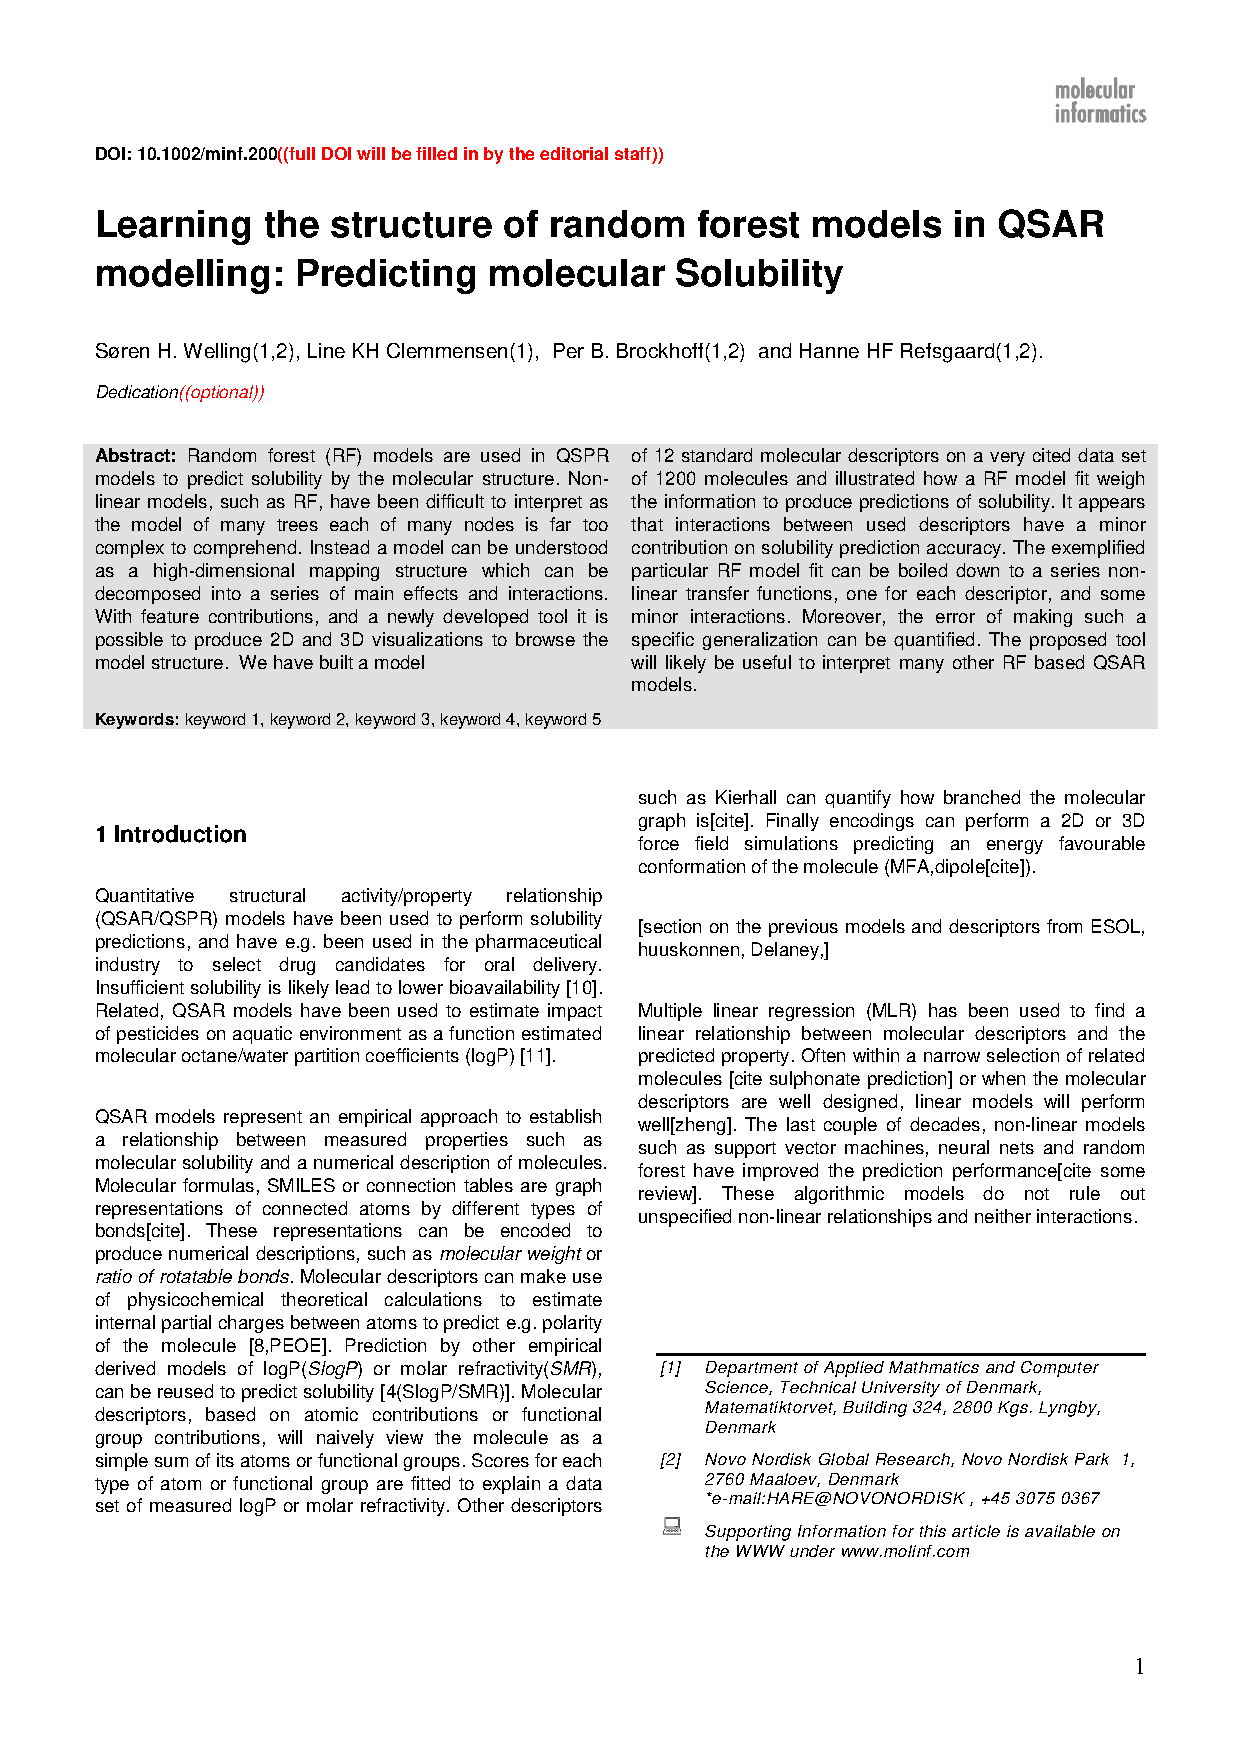
\includepdf[pages={1-},scale=0.90,pagecommand={\pagestyle{myruled}}]{appendices/structureOfSolubility.pdf}

\section{Random forest Q and A answers with illustrations and code examples}

During the last three years, two forums \textit{Stack Overflow} \url{http://stackoverflow.com/} for learning programming and \textit{Cross Validated} \url{stats.stackexchange.com} for learning statistics have been invaluable daily sources of fast answers to questions on all levels. Whenever you get stuck and that probably happens 10 times a day, you only have to complain to google about the problem in a sentence. As we are six billions on this planet, odds are favorable for, that some person on the same level already has had this problem before. This person posed the same question in the same silly wording as you do now, and some helpful person has already answered with a practical example, and perhaps also provided answers to other question, you really ought to be asking instead. The cross validated site is relatively small with only 83,000 questions (July 2016), where \textit{Stack Overflow} has 12,000,000 questions to cover most programming languages. For the entertainment value and to test my knowledge on random forest, I started to answer questions my self. By putting my beliefs on public display, I sometimes receive swift criticism, when I was wrong. I have answered 92 questions. Each answer required in average a page and often comprises visulizations, coding, references to other material and took a half to 3 hours to write. I have included some of my favorite answers here, and have referred to these through this thesis. The cross-validated site has almost 100.000 users, and reputation voting wise, I rank top 200. My answers have presently in total 75,000 page views (~50.000 views/yr), which is probably some 4 orders of magnitude more than this chapter ever will be read.


\subsection{Handling unbalanced data with with random forest}
\label{CV1_classwt}
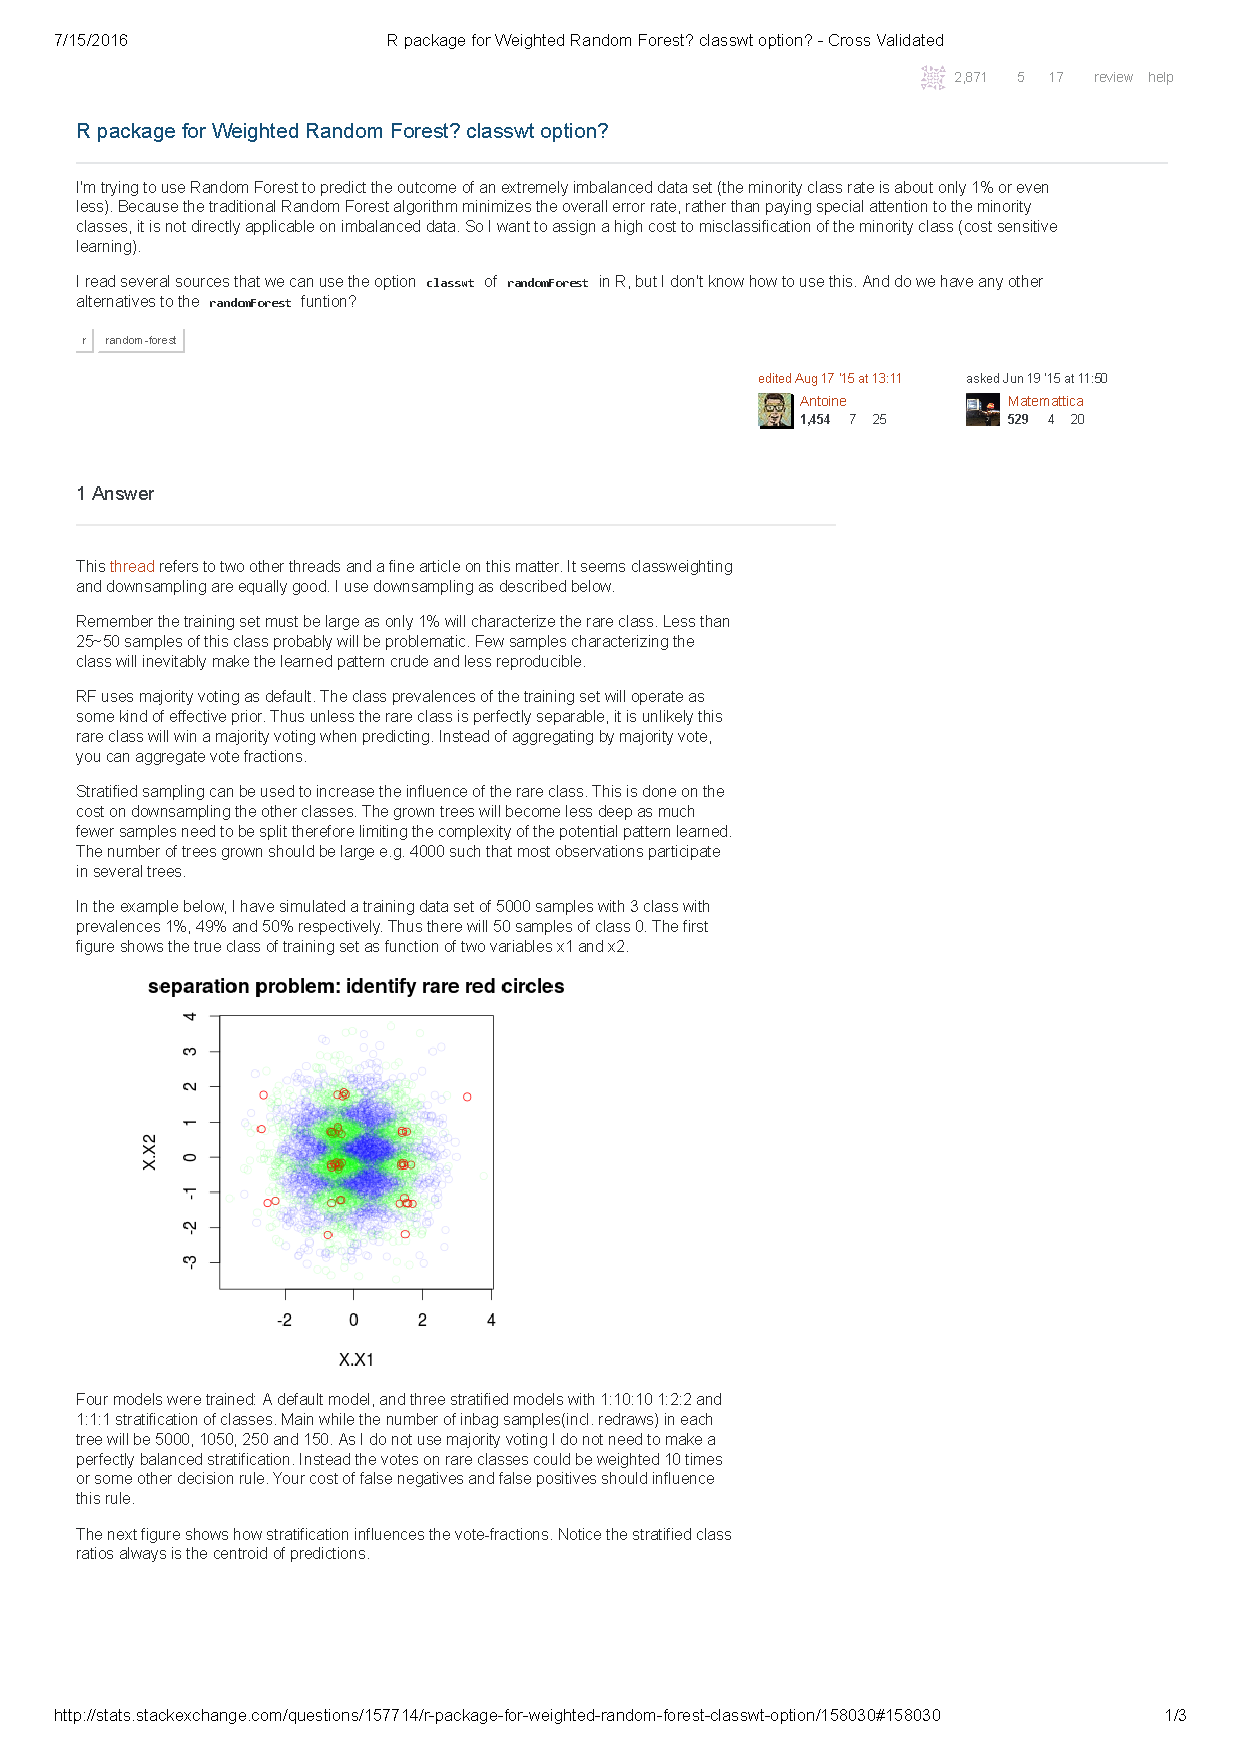
\includepdf[pages={1-},scale=0.90,offset=0 -34, pagecommand={\pagestyle{myruled}}]{cross_validated_posts/CV1_classwt.pdf}


\subsection{Random forest and outliers I: Outlier Islands}
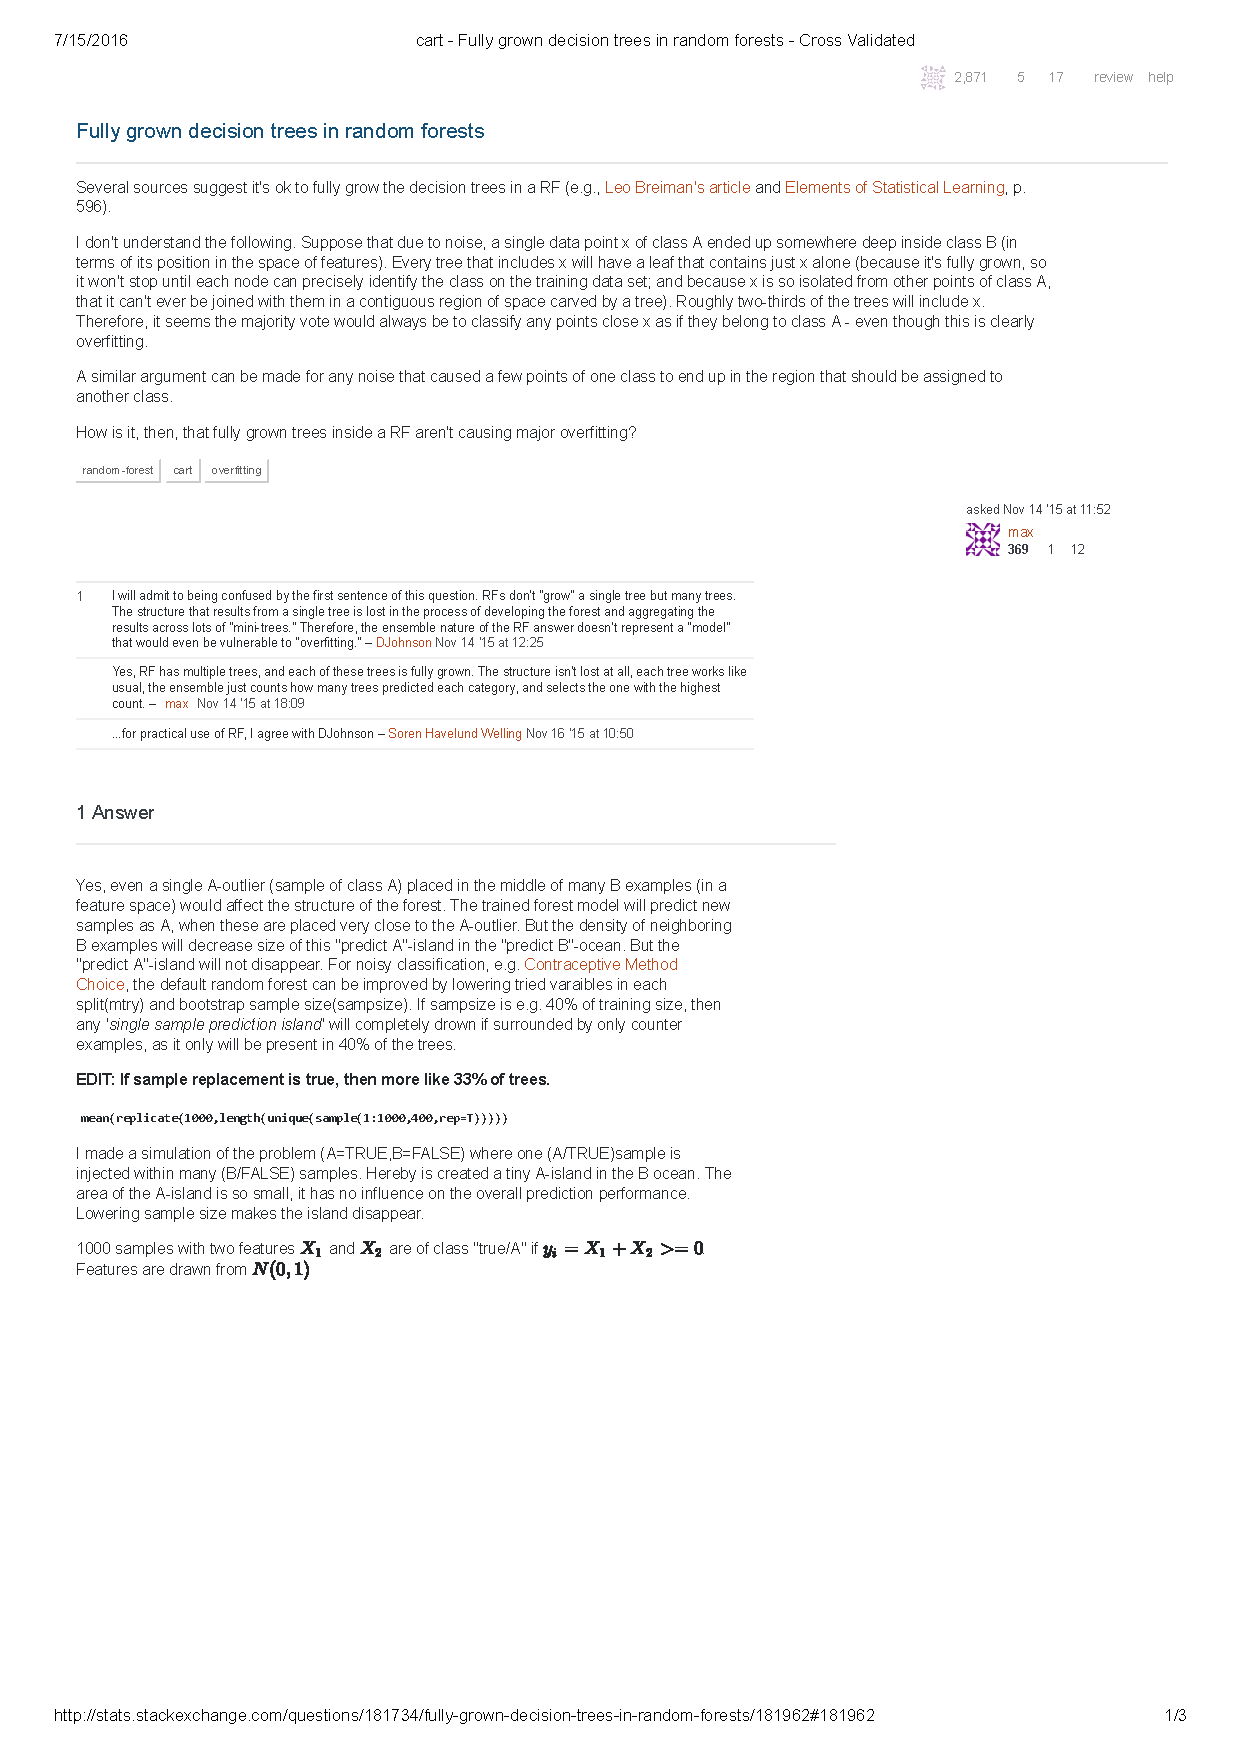
\includepdf[pages={1-},scale=0.90,offset=0 -34, pagecommand={\pagestyle{myruled}}]{cross_validated_posts/CV2_fullygrown.pdf}
\label{CV2_fullygrown}

\subsection{Random forest and outliers II: Robustness}
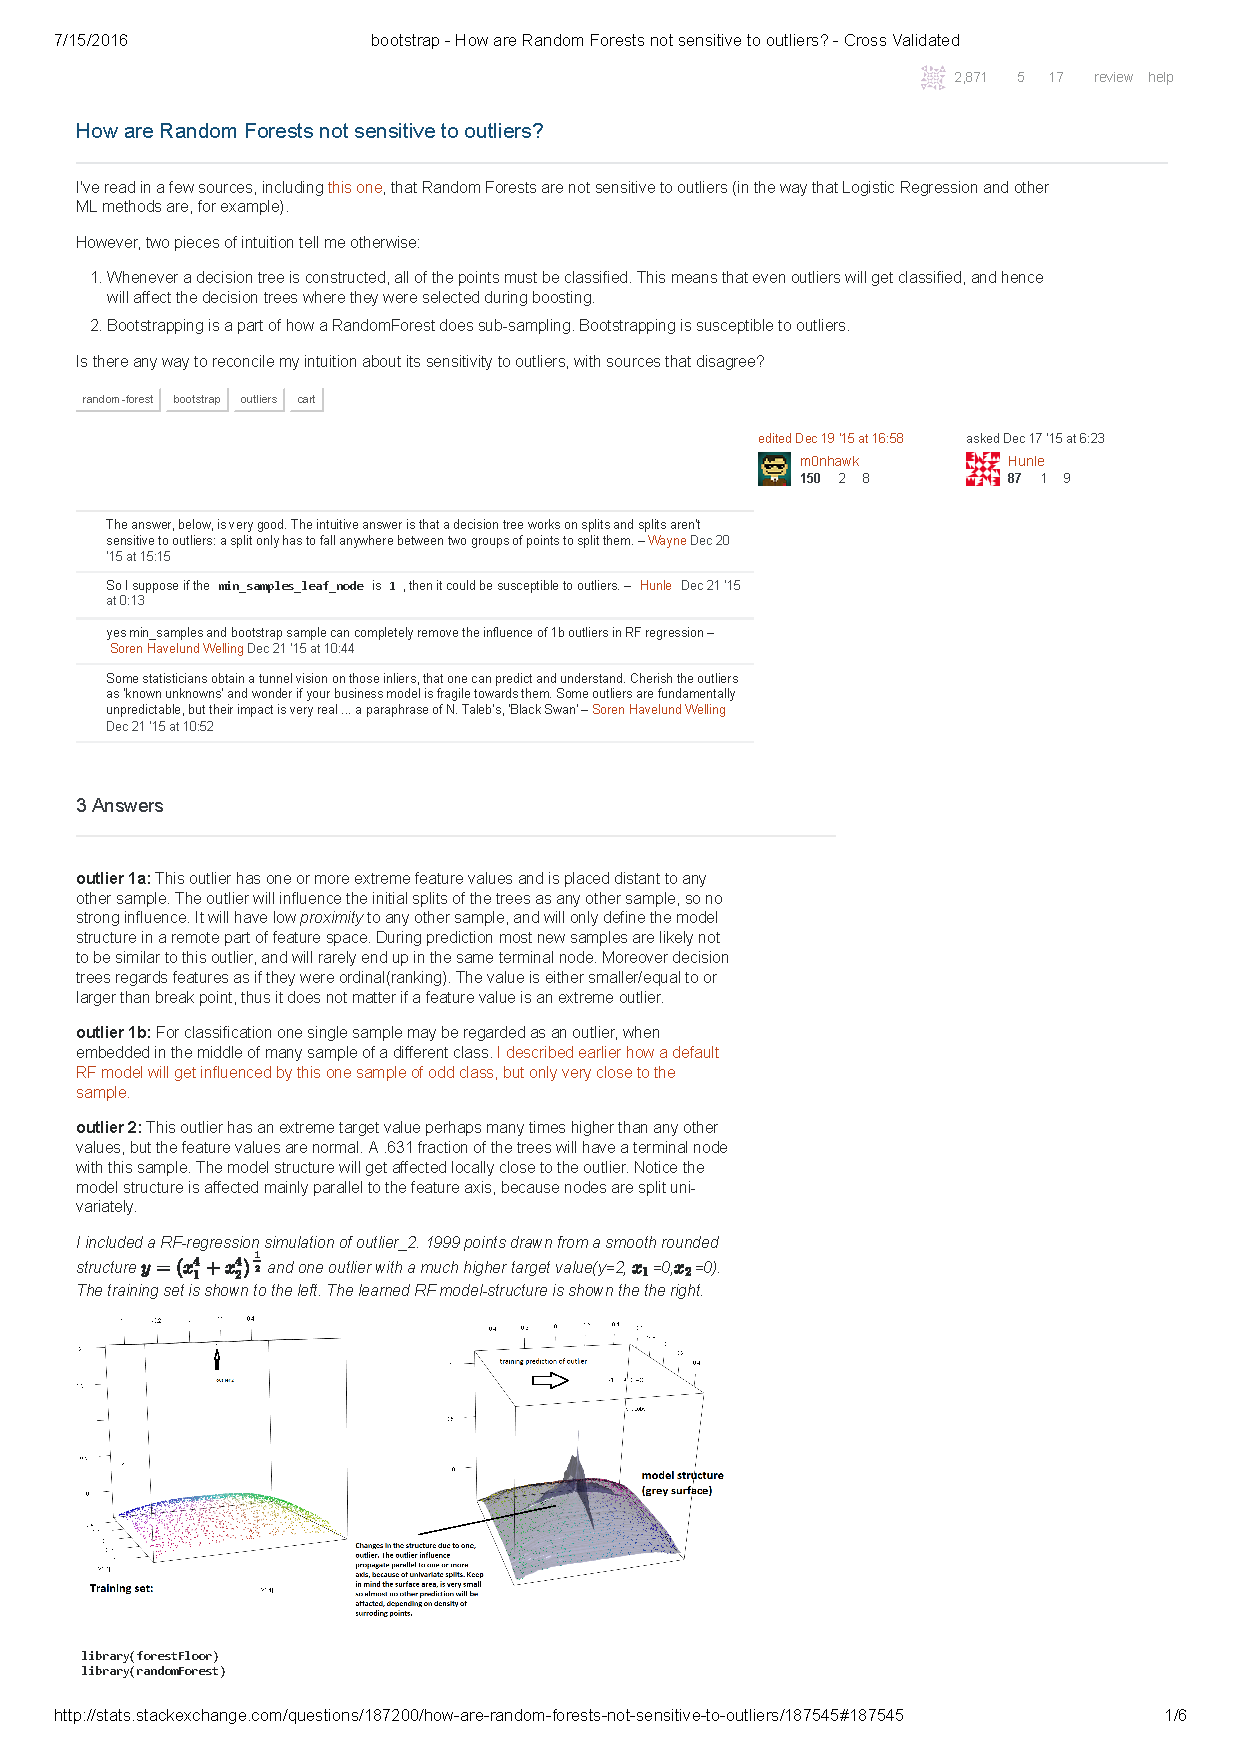
\includepdf[pages={1-},scale=0.90,offset=0 -34, pagecommand={\pagestyle{myruled}}]{cross_validated_posts/CV3_sensitiveOutliers.pdf}
\label{CV3_sensitiveOutliers}

\subsection{Simple check that random forest can fit interactions}
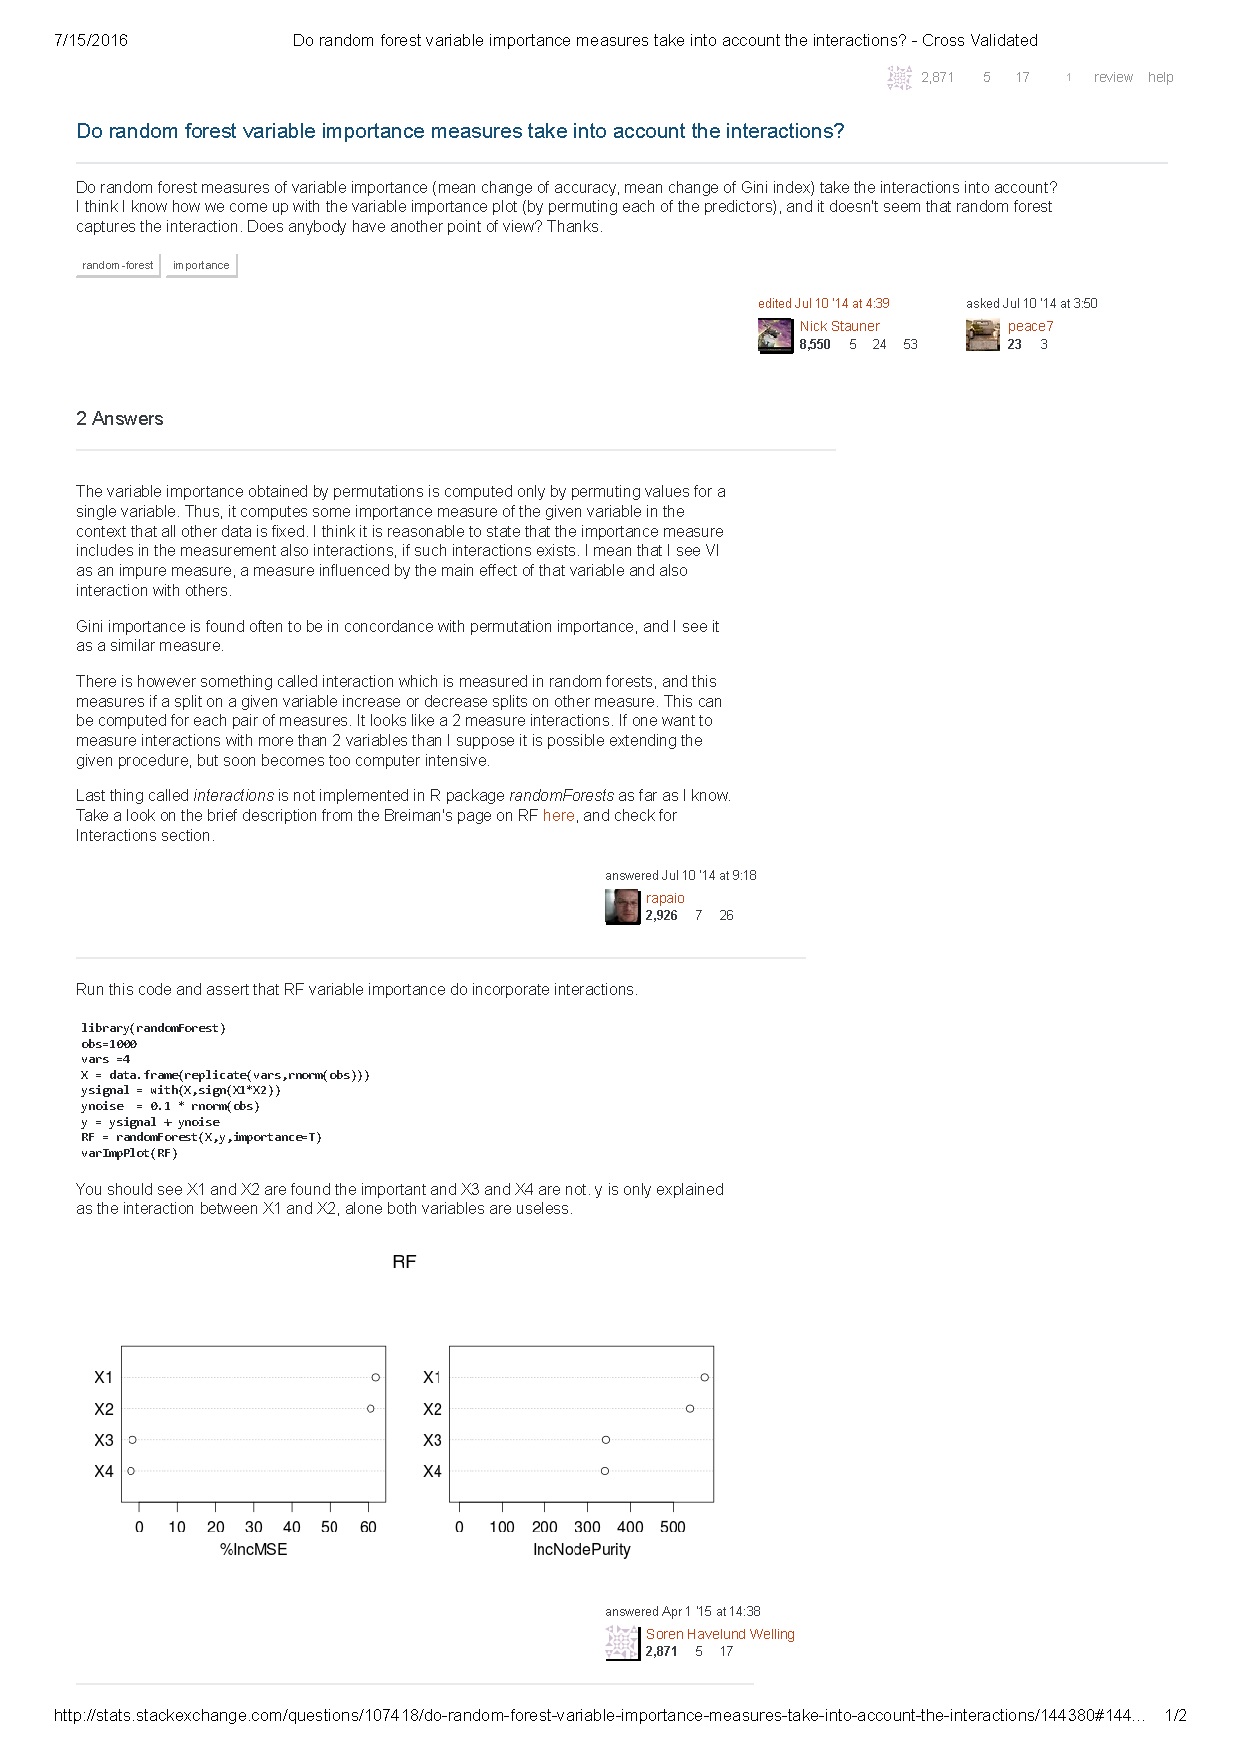
\includepdf[pages={1-},scale=0.90,offset=0 -34, pagecommand={\pagestyle{myruled}}]{cross_validated_posts/CV4_assertInteraction.pdf}
\label{CV4_assertInteraction}

\subsection{Interpolation with RF and SVM is very similar. Extrapolation is not.}
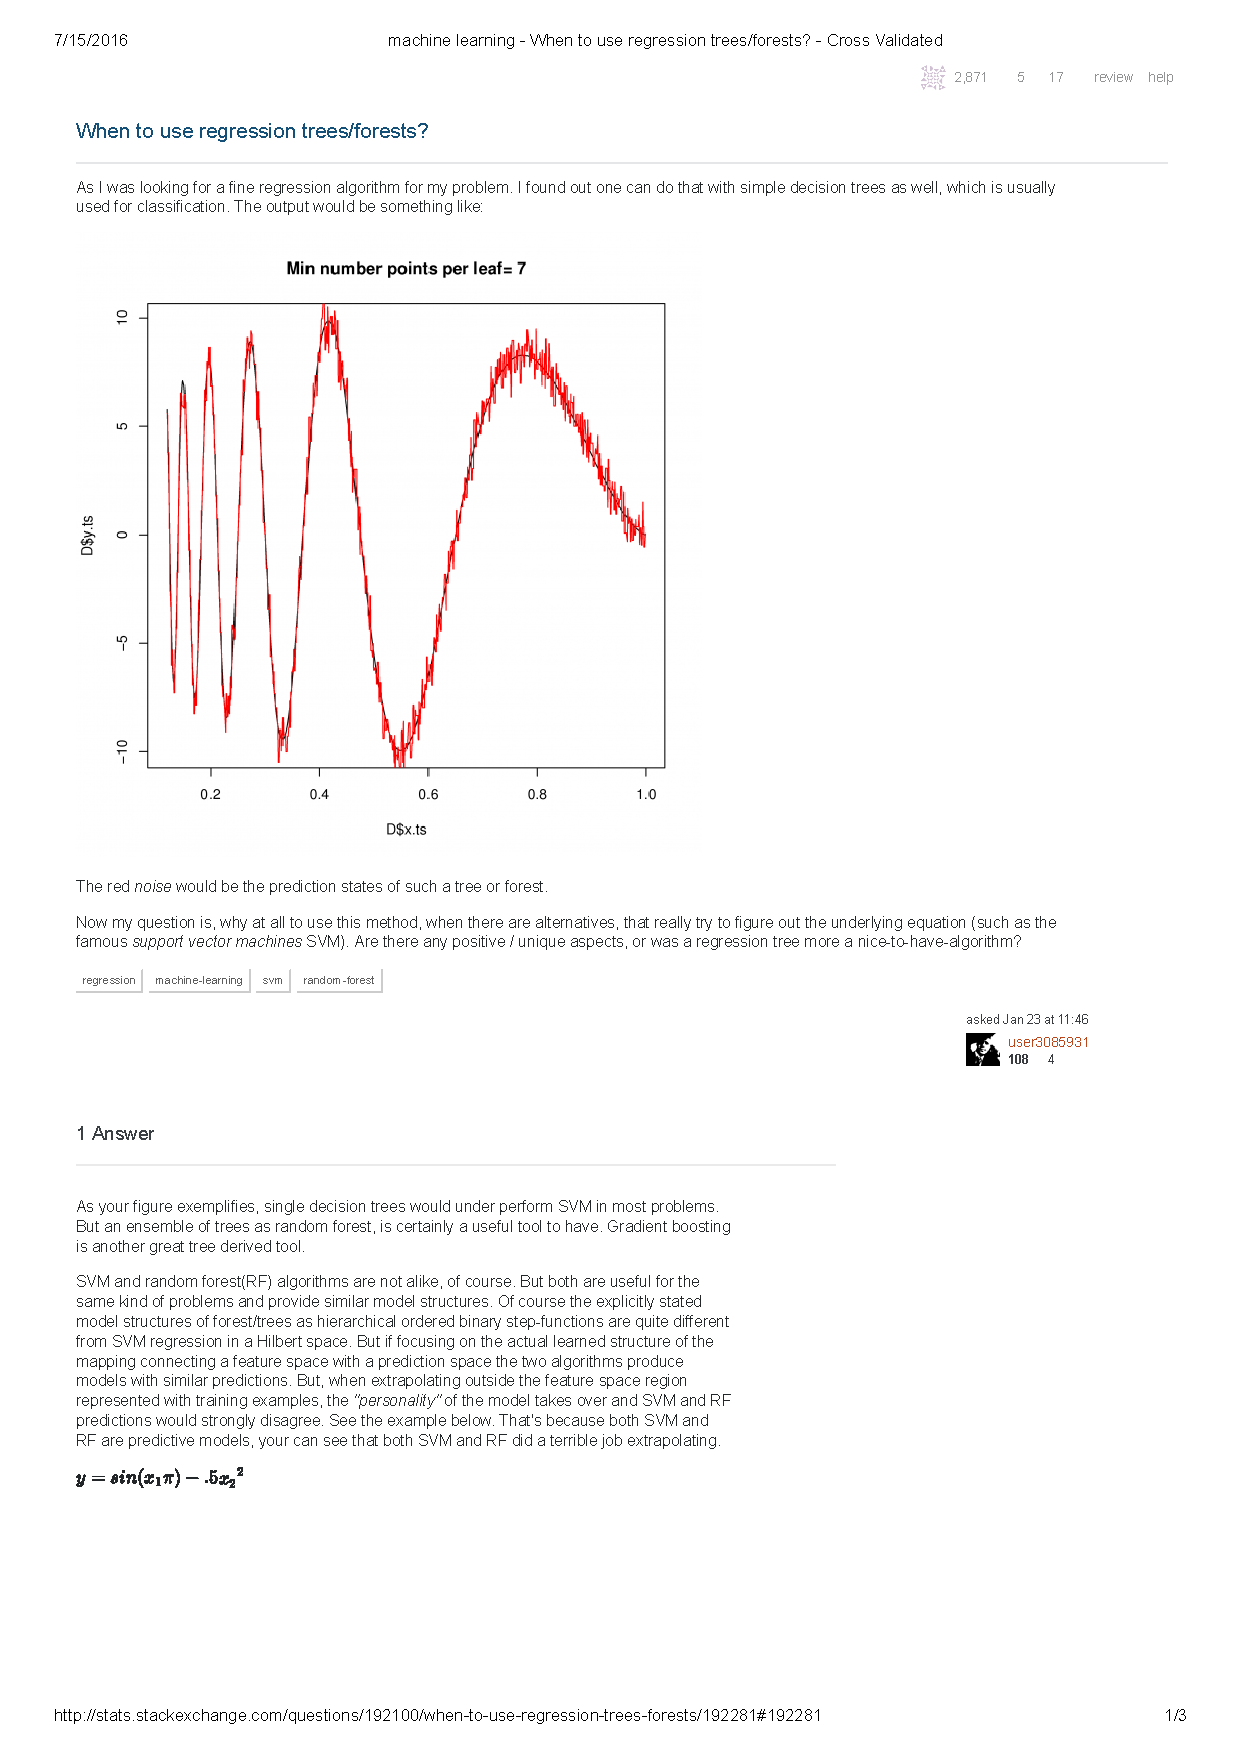
\includepdf[pages={1-},scale=0.90,offset=0 -34, pagecommand={\pagestyle{myruled}}]{cross_validated_posts/CV5_SVM_RF_same_same.pdf}
\label{CV5_SVM_RF_same_same}

\subsection{How does CART break ties}
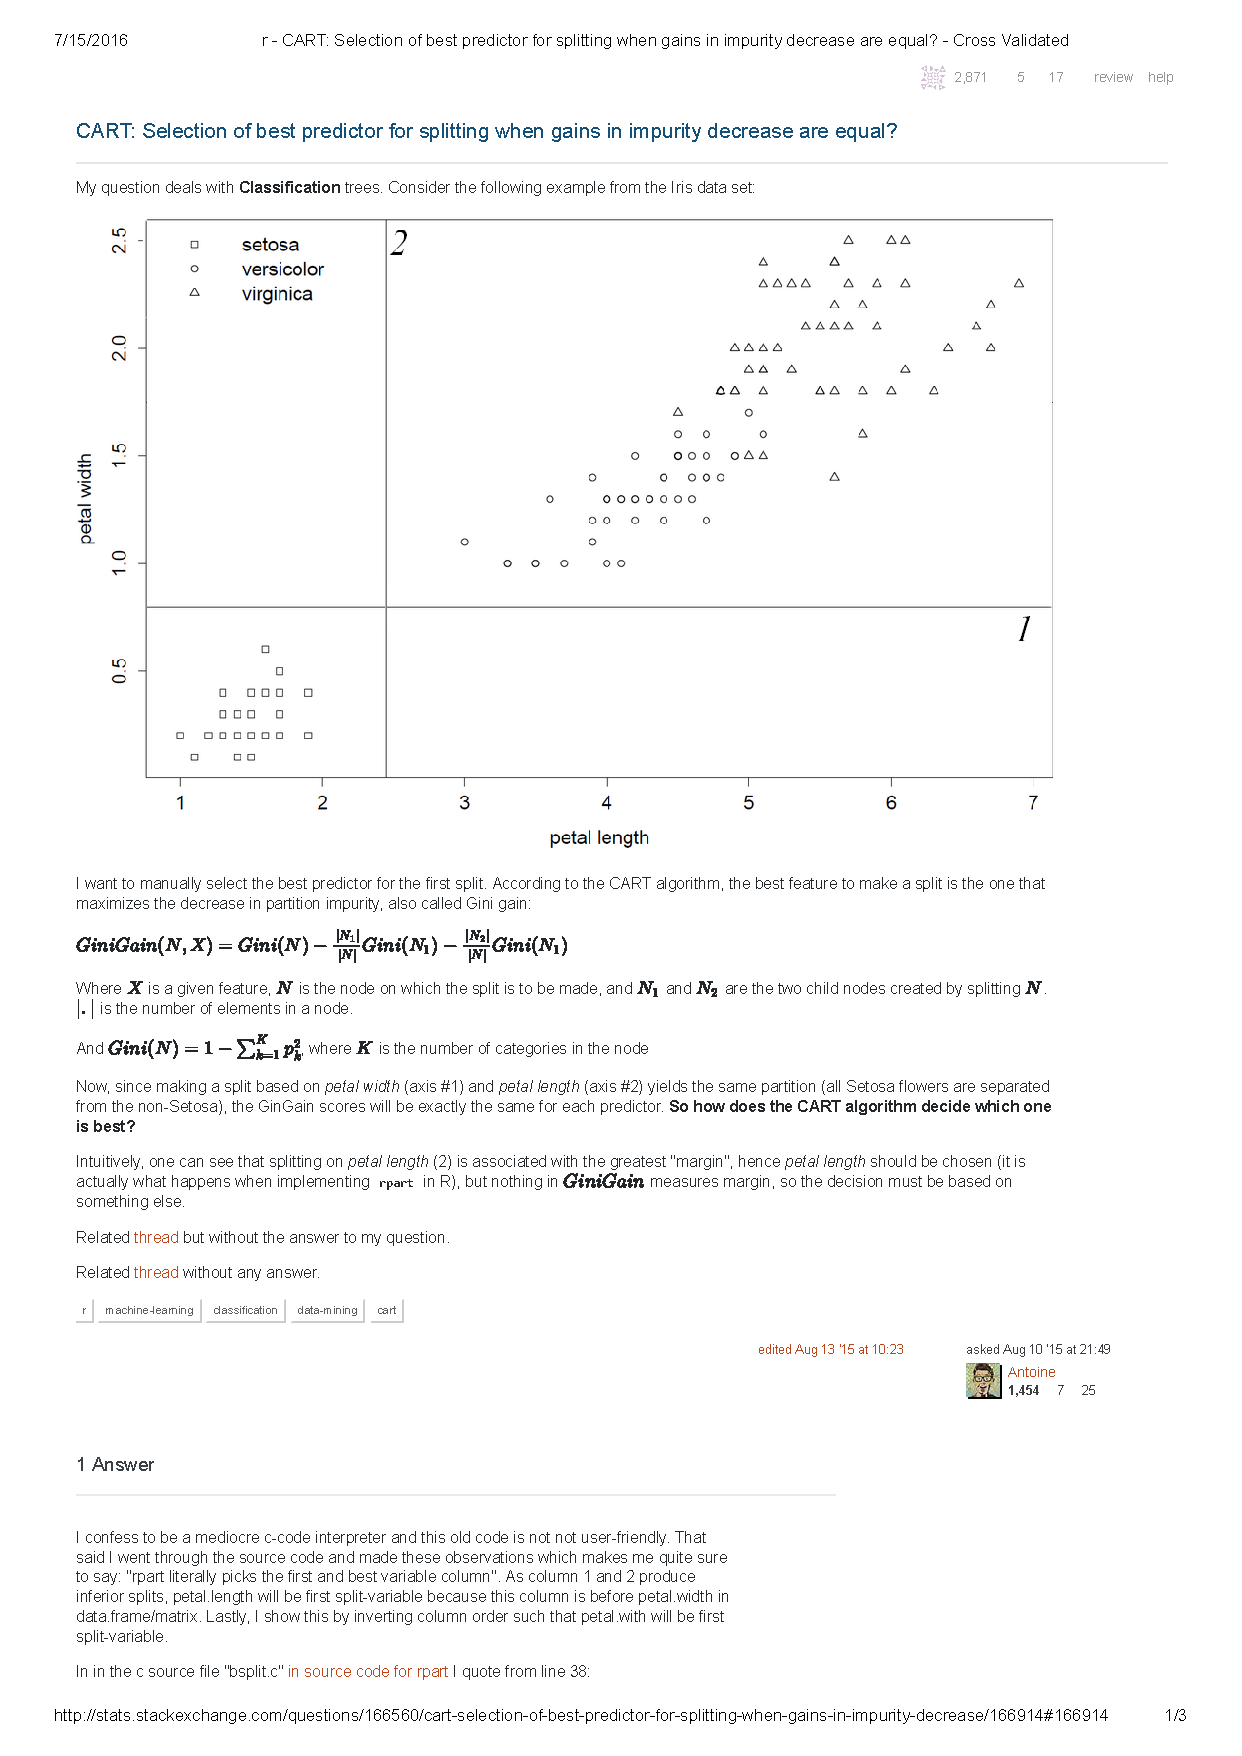
\includepdf[pages={1-},scale=0.90,offset=0 -34, pagecommand={\pagestyle{myruled}}]{cross_validated_posts/CV6_CARTtiebreak.pdf}
\label{CV6_CARTtiebreak}

\subsection{Variable importance for other models than random forest}
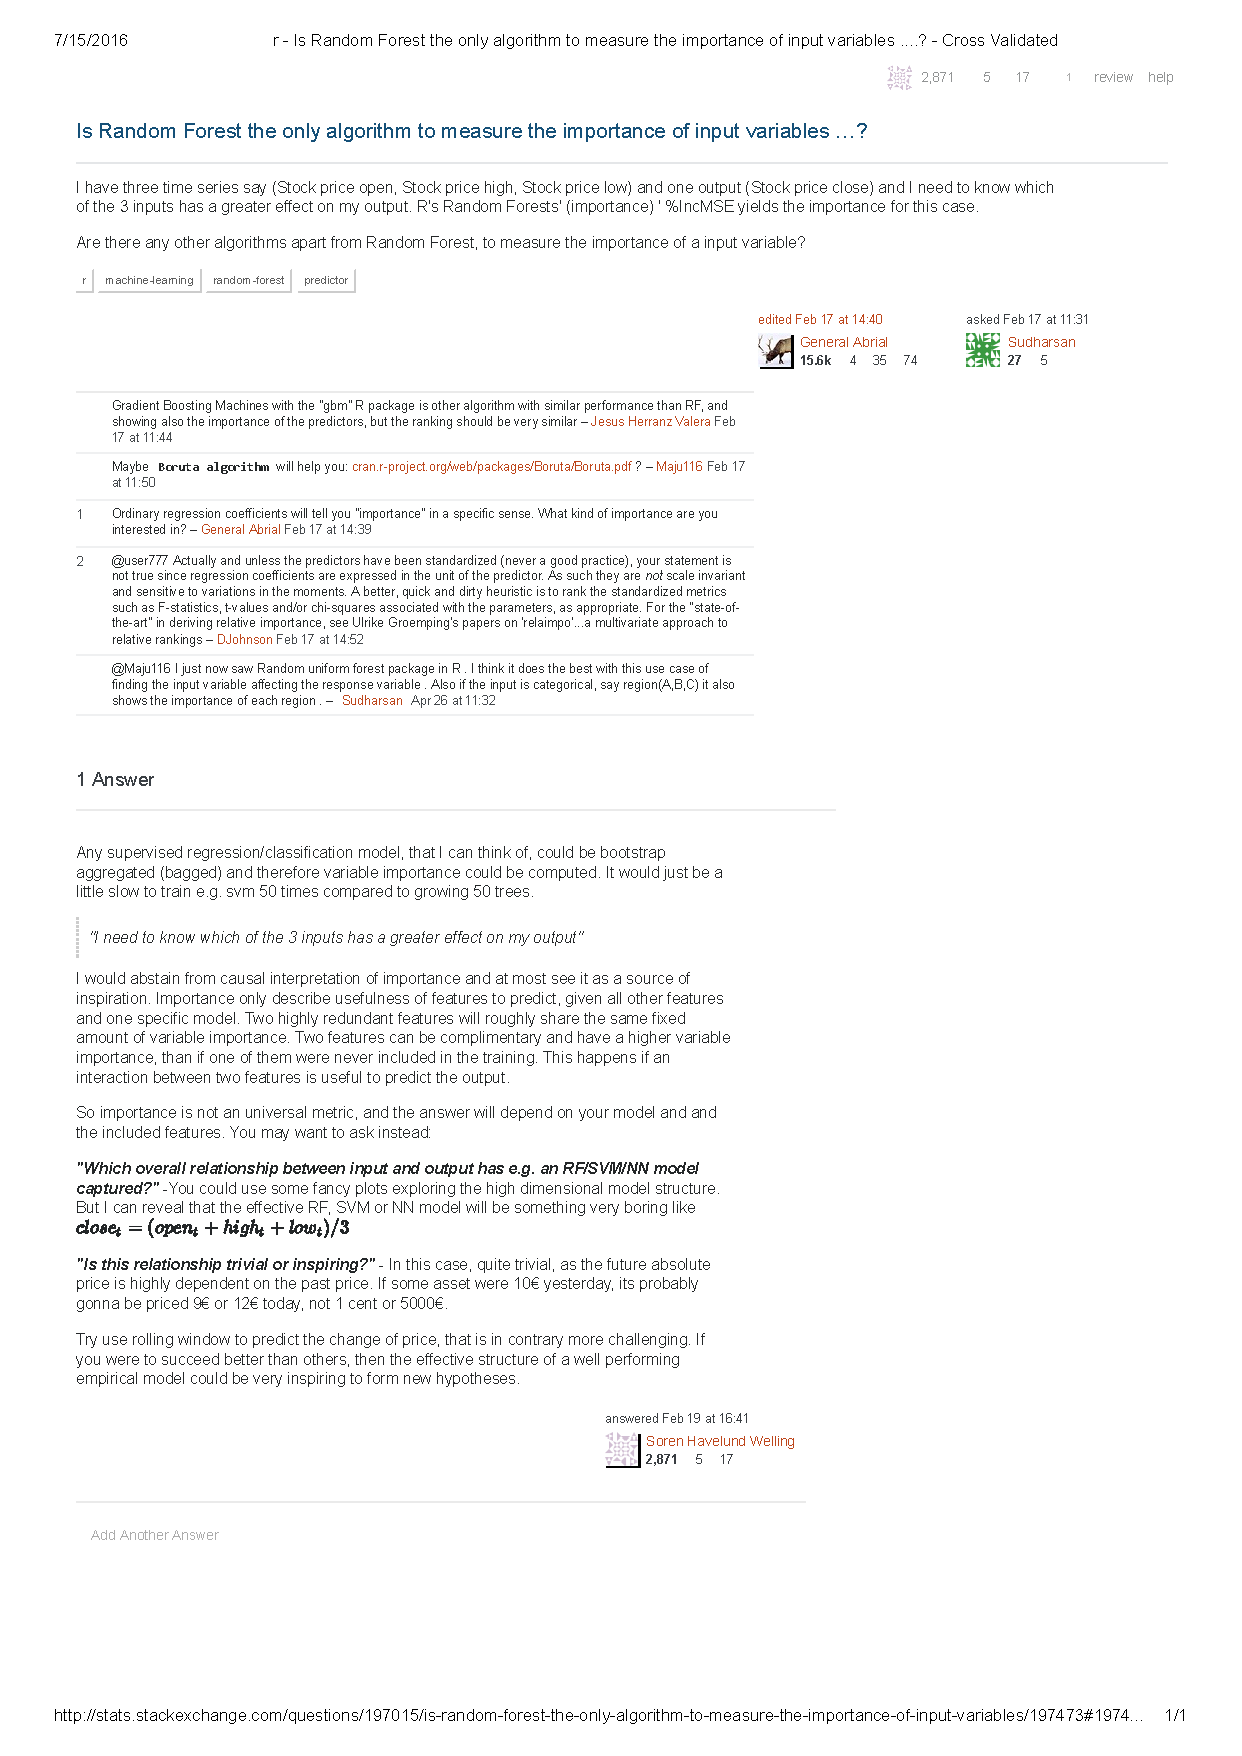
\includepdf[pages={1-},scale=0.90,offset=0 -34, pagecommand={\pagestyle{myruled}}]{cross_validated_posts/CV7_VIbeyondRF.pdf}
\label{CV7_VIbeyondRF}

\subsection{How to combine multiple models in a bootstrap aggregated ensemble}
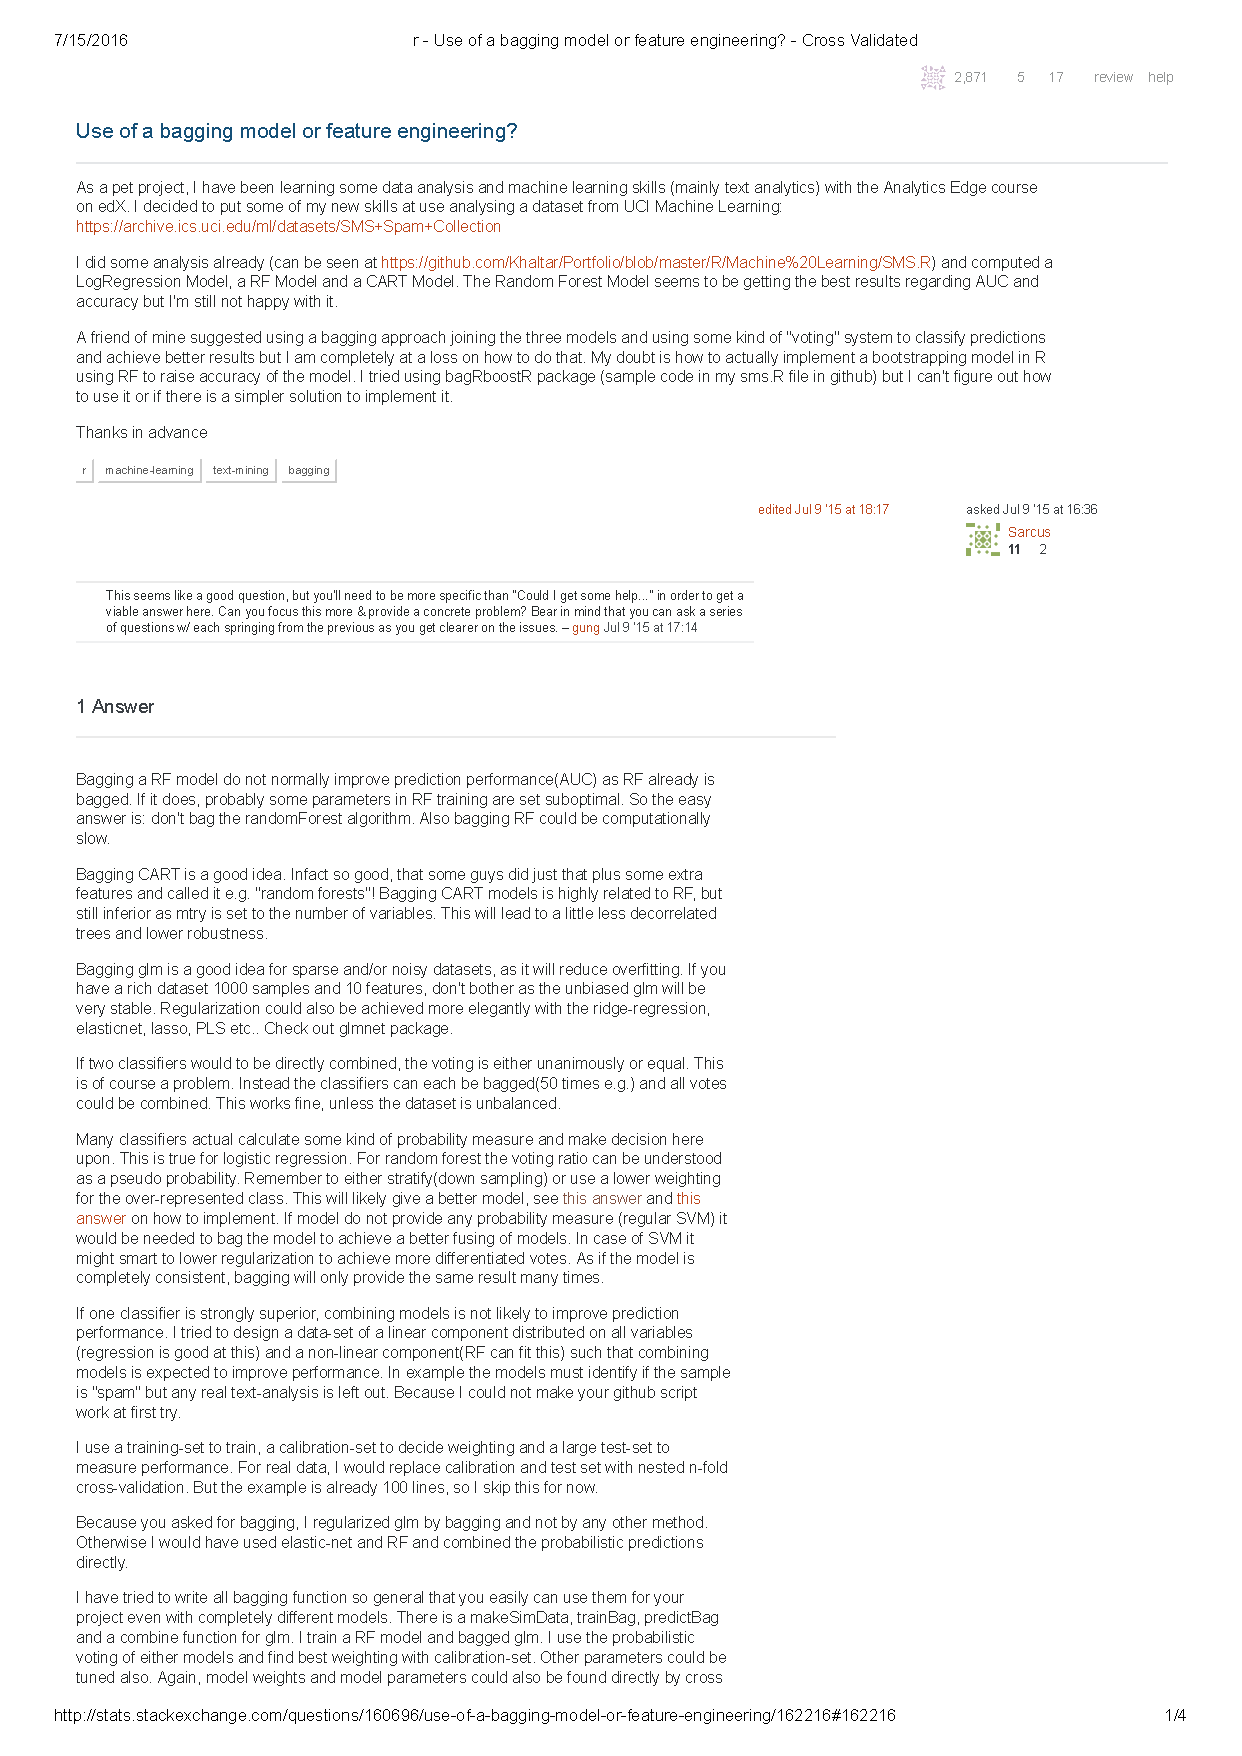
\includepdf[pages={1-},scale=0.90,offset=0 -34, pagecommand={\pagestyle{myruled}}]{cross_validated_posts/CV8_combineBagging}
\label{CV8_combineBagging}

\subsection{Bootstrapping process of random forest: Sampling proability as function of hyperparameters.}
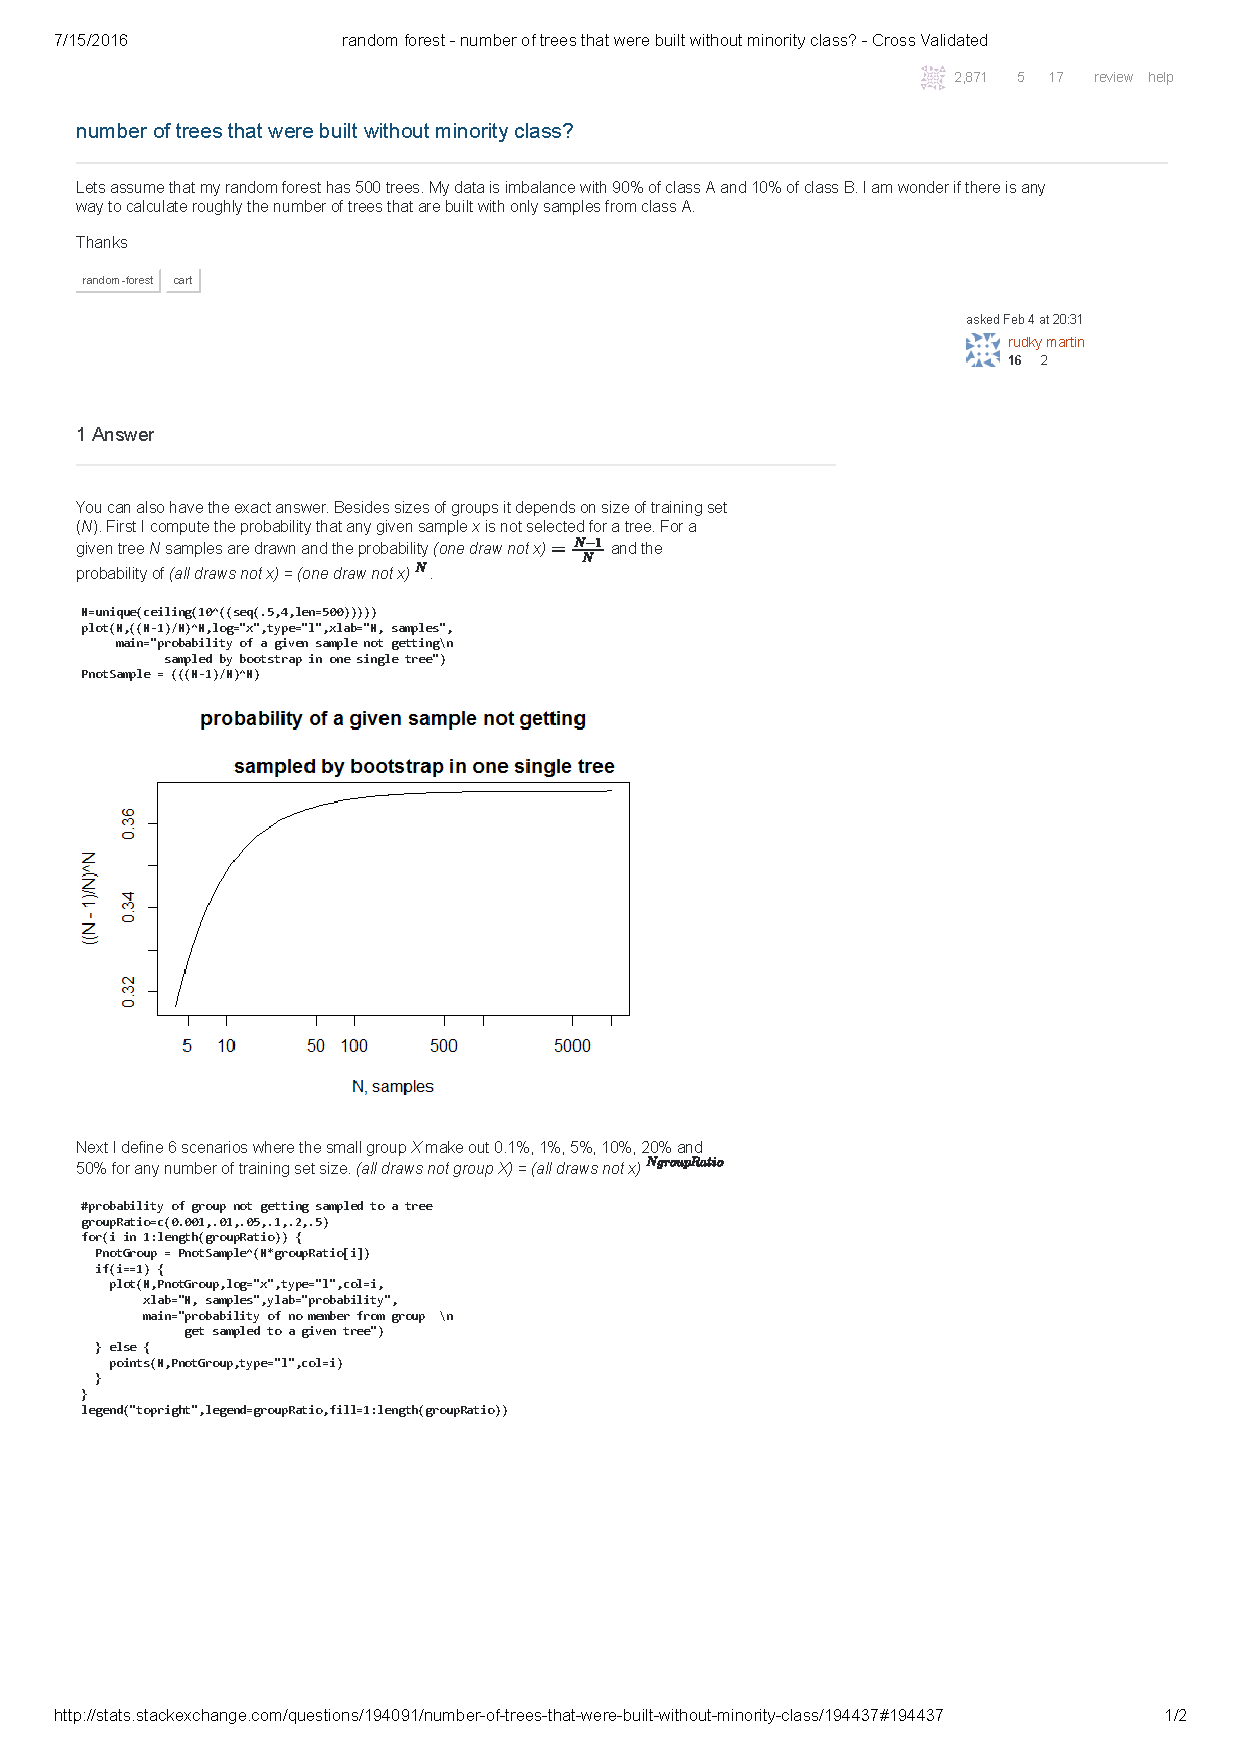
\includepdf[pages={1-},scale=0.90,offset=0 -34, pagecommand={\pagestyle{myruled}}]{cross_validated_posts/CV9_RFsampling}
\label{CV9_RFsampling}

\subsection{Simple tutorial on log transformation before PCA}
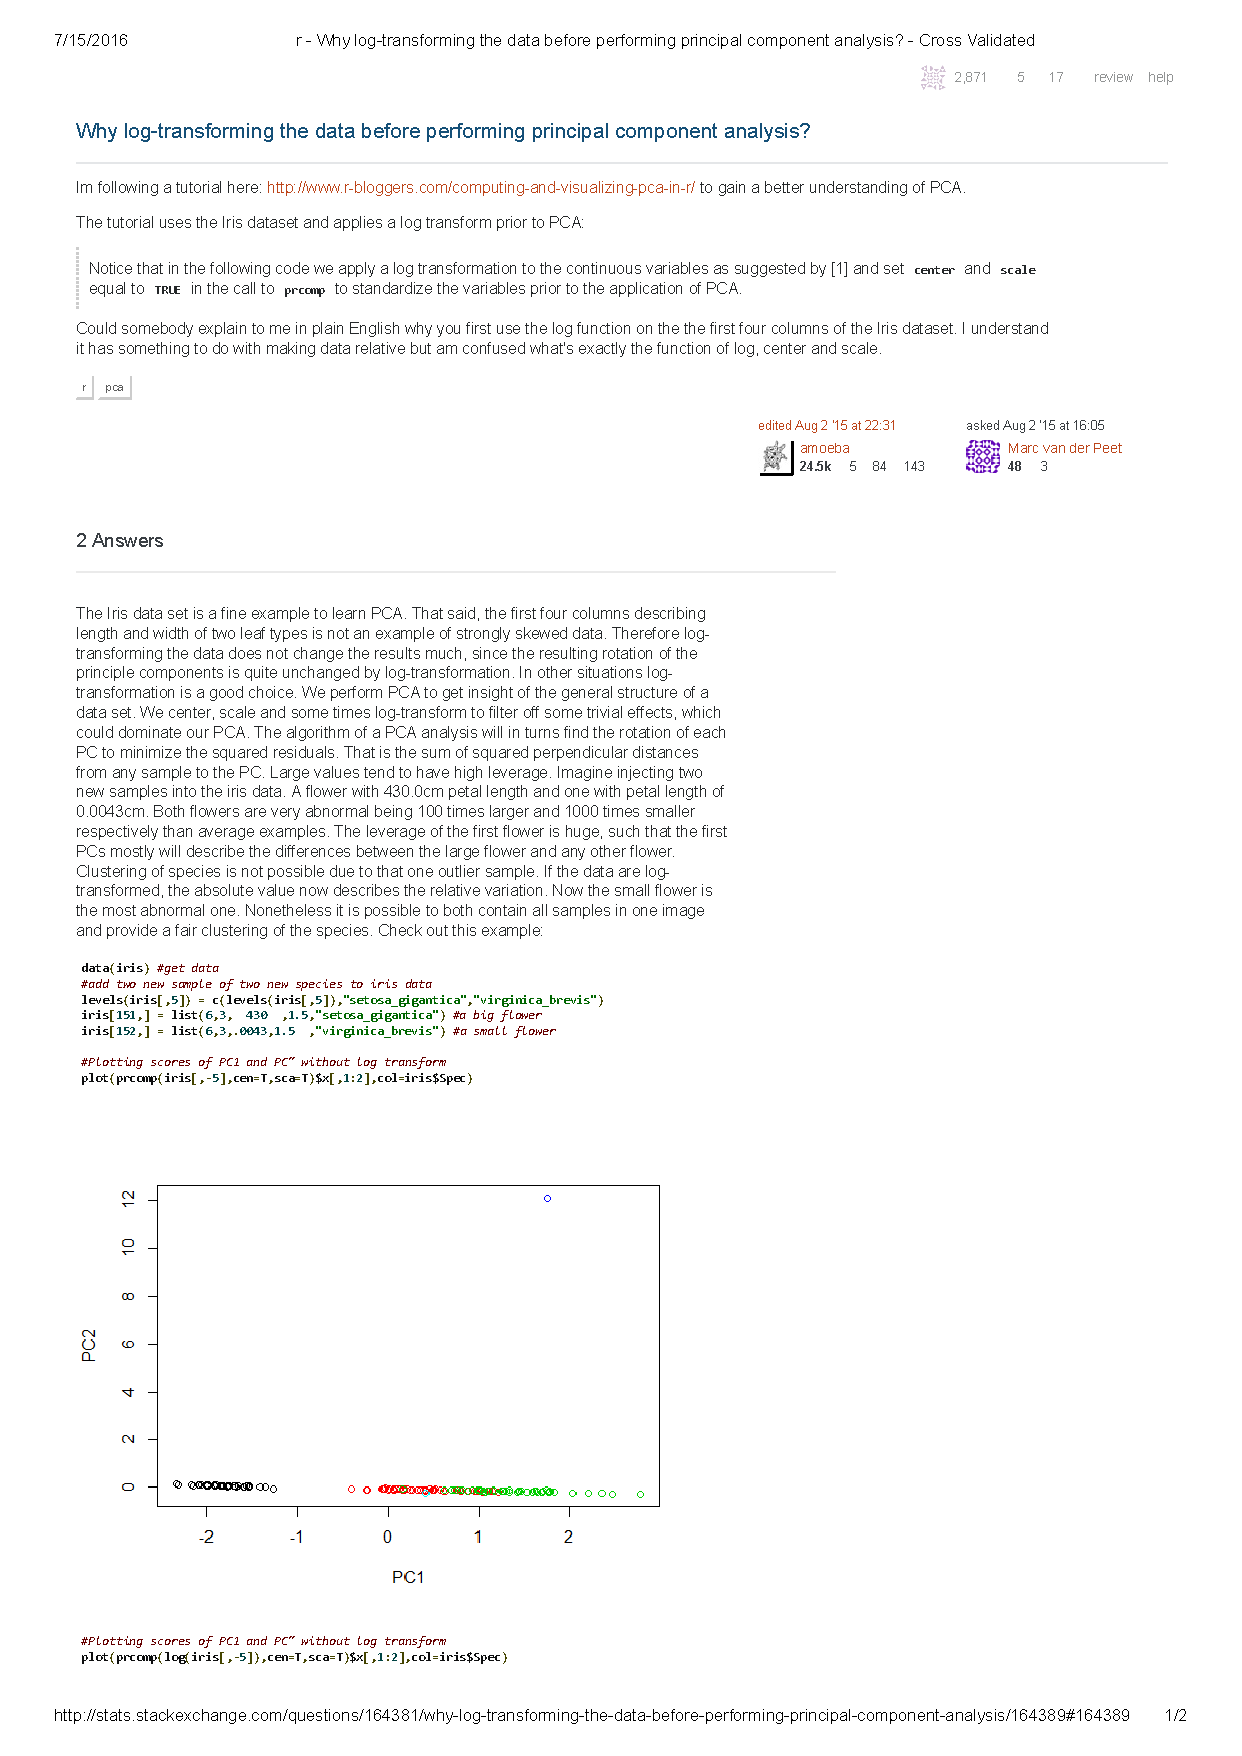
\includepdf[pages={1-},scale=0.90,offset=0 -34, pagecommand={\pagestyle{myruled}}]{cross_validated_posts/CV10_PCAlogTransform}
\label{CV10_PCAlogTransform}

\subsection{Efficient implementation gini loss function in random forest}
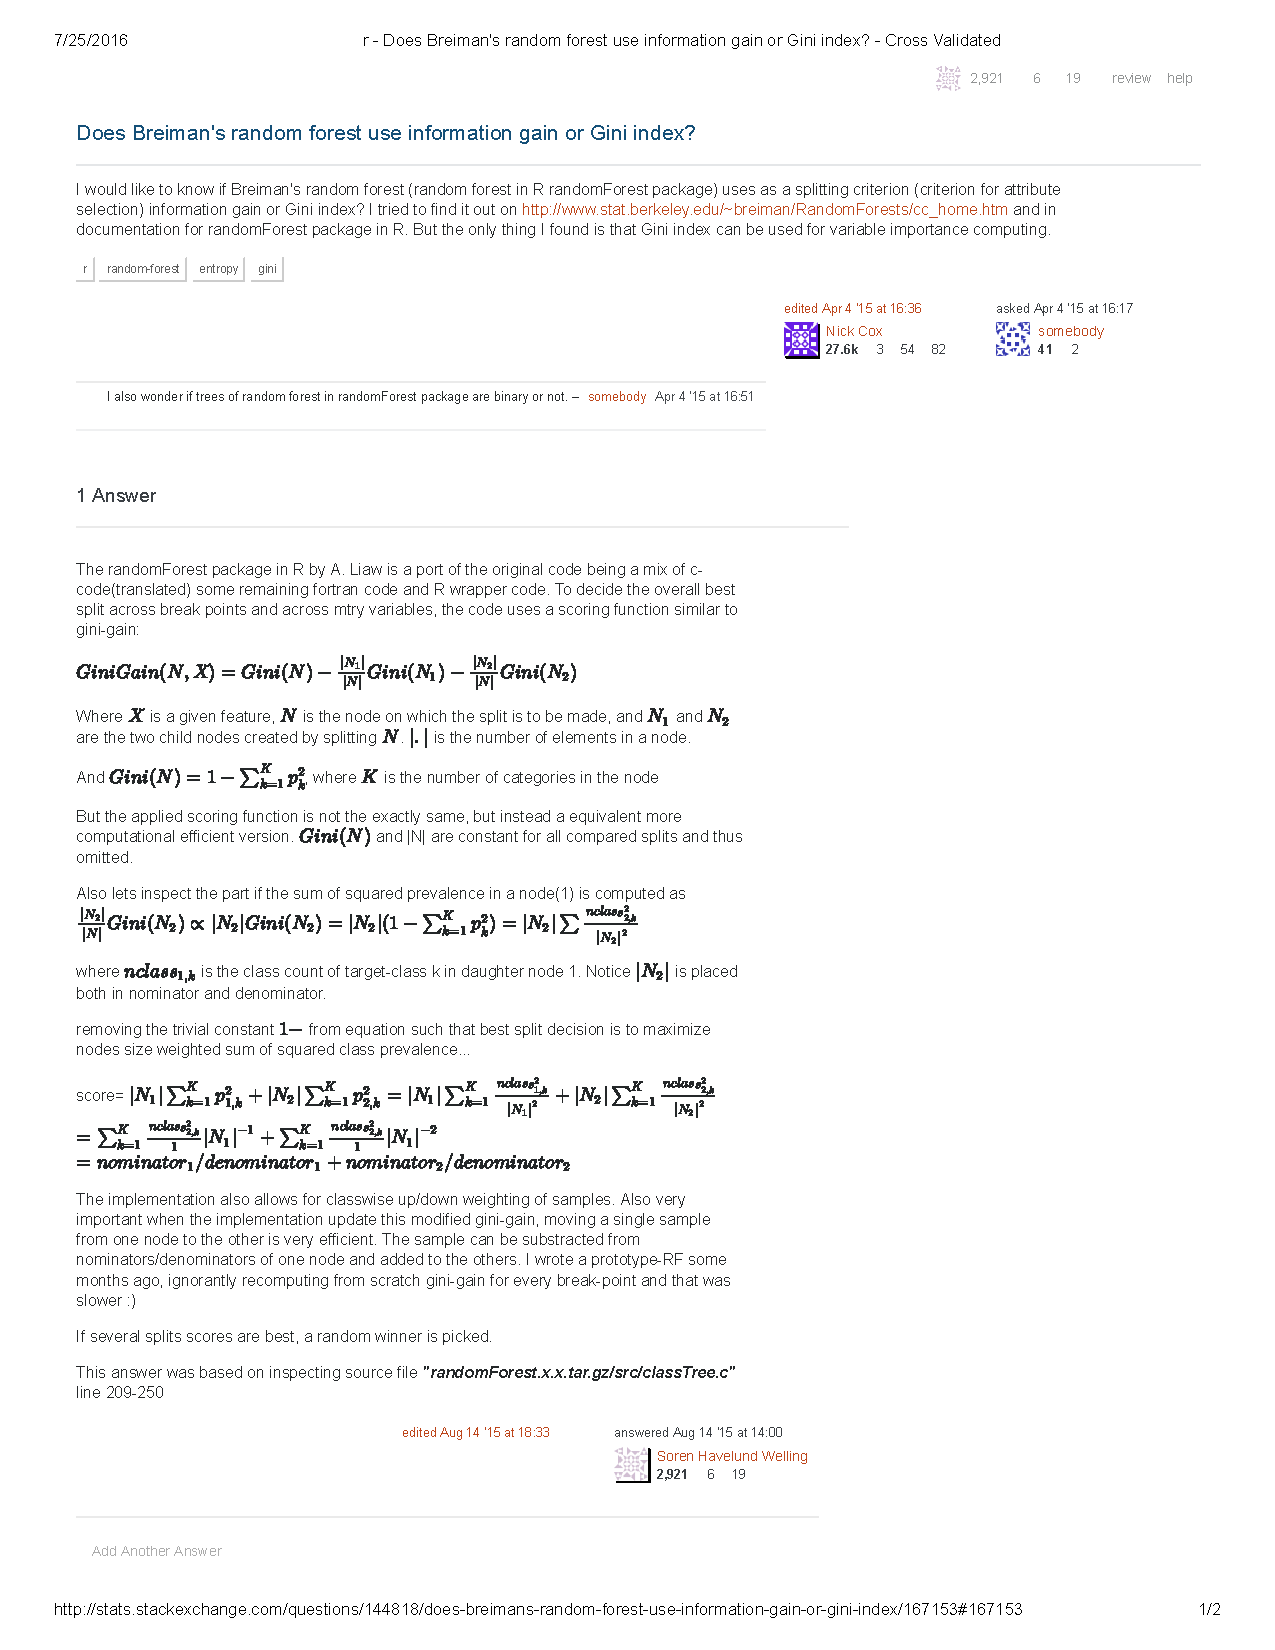
\includepdf[pages={1-},scale=0.90,offset=0 -34, pagecommand={\pagestyle{myruled}}]{cross_validated_posts/CV11_RFginigain.pdf}
\label{CV11_RFginigain}

\subsection{Limiting bootstrap sample size versus limiting maxnodes}
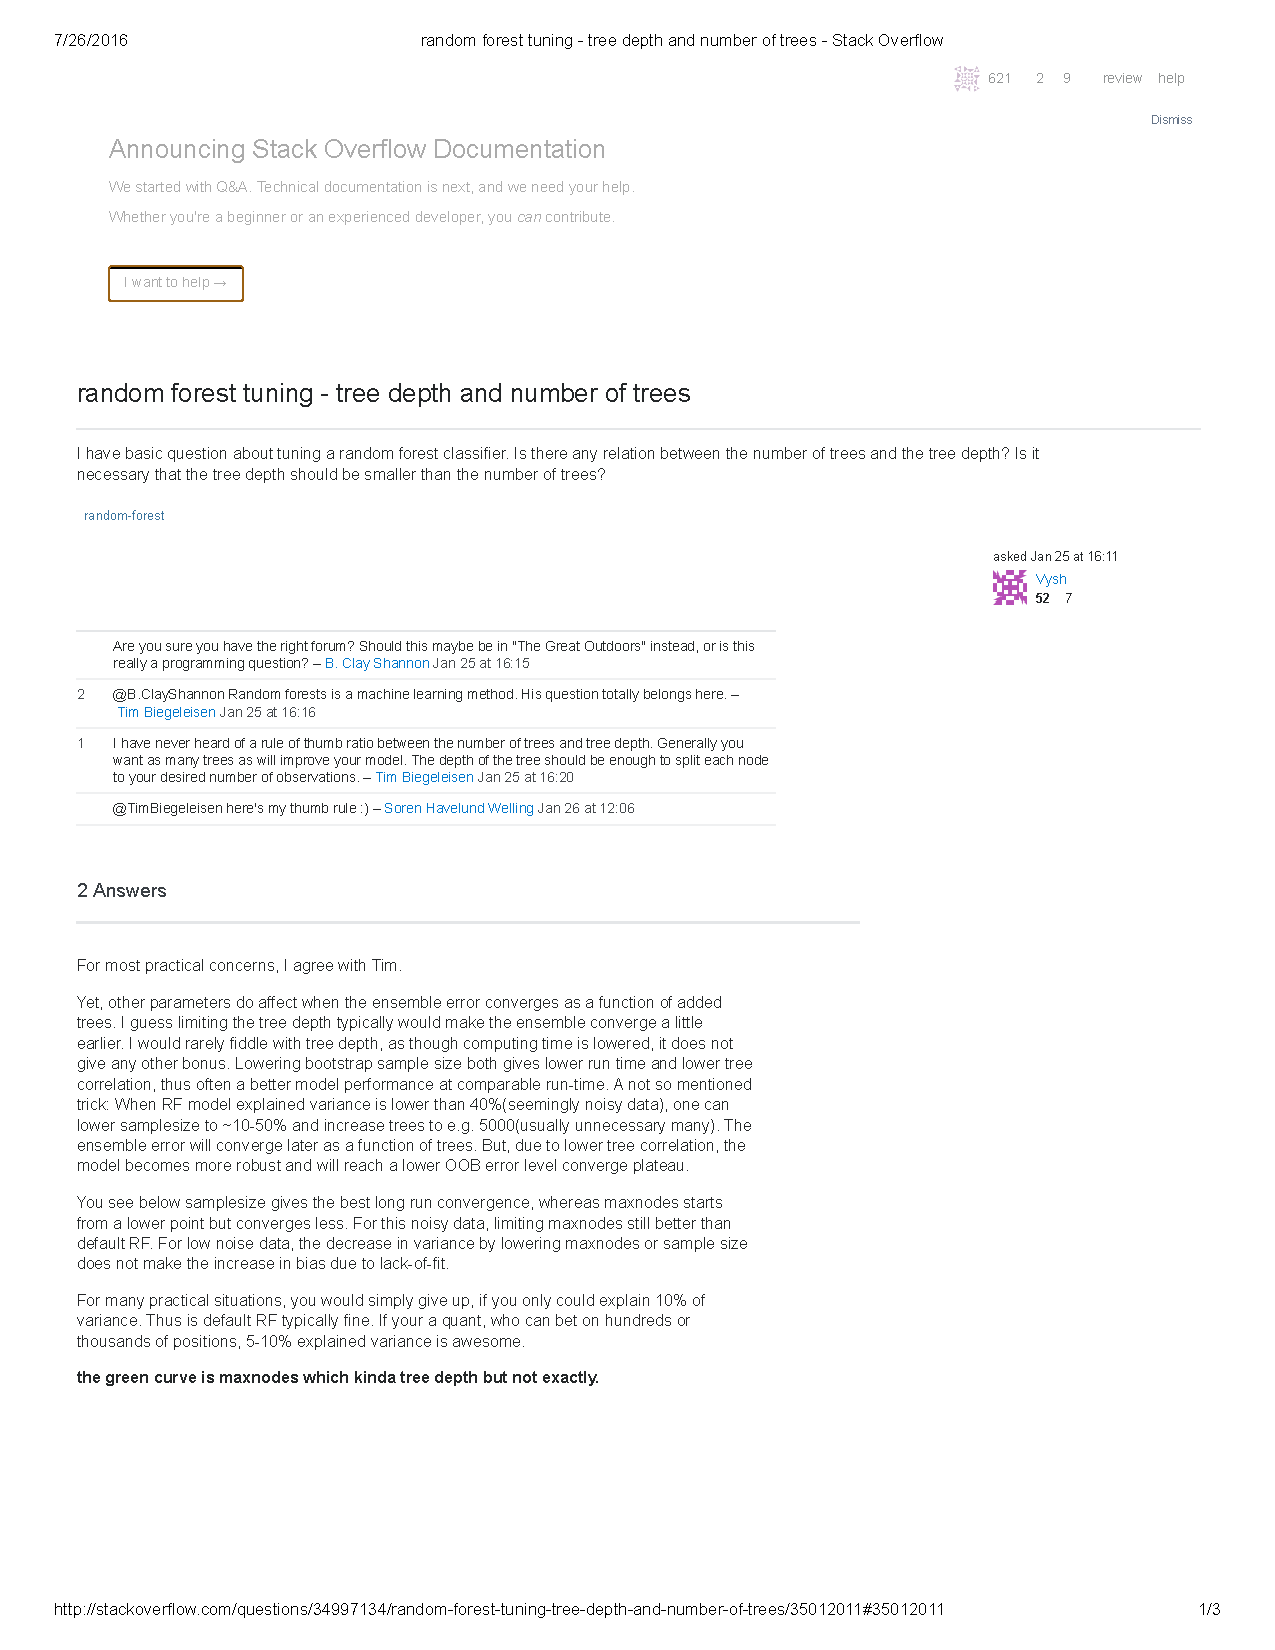
\includepdf[pages={1-},scale=0.90,offset=0 -34, pagecommand={\pagestyle{myruled}}]{cross_validated_posts/CV12_RFsampsize.pdf}
\label{CV12_RFsampsize}


\section{Manual: R CRAN package forestFloor 1.9.5}

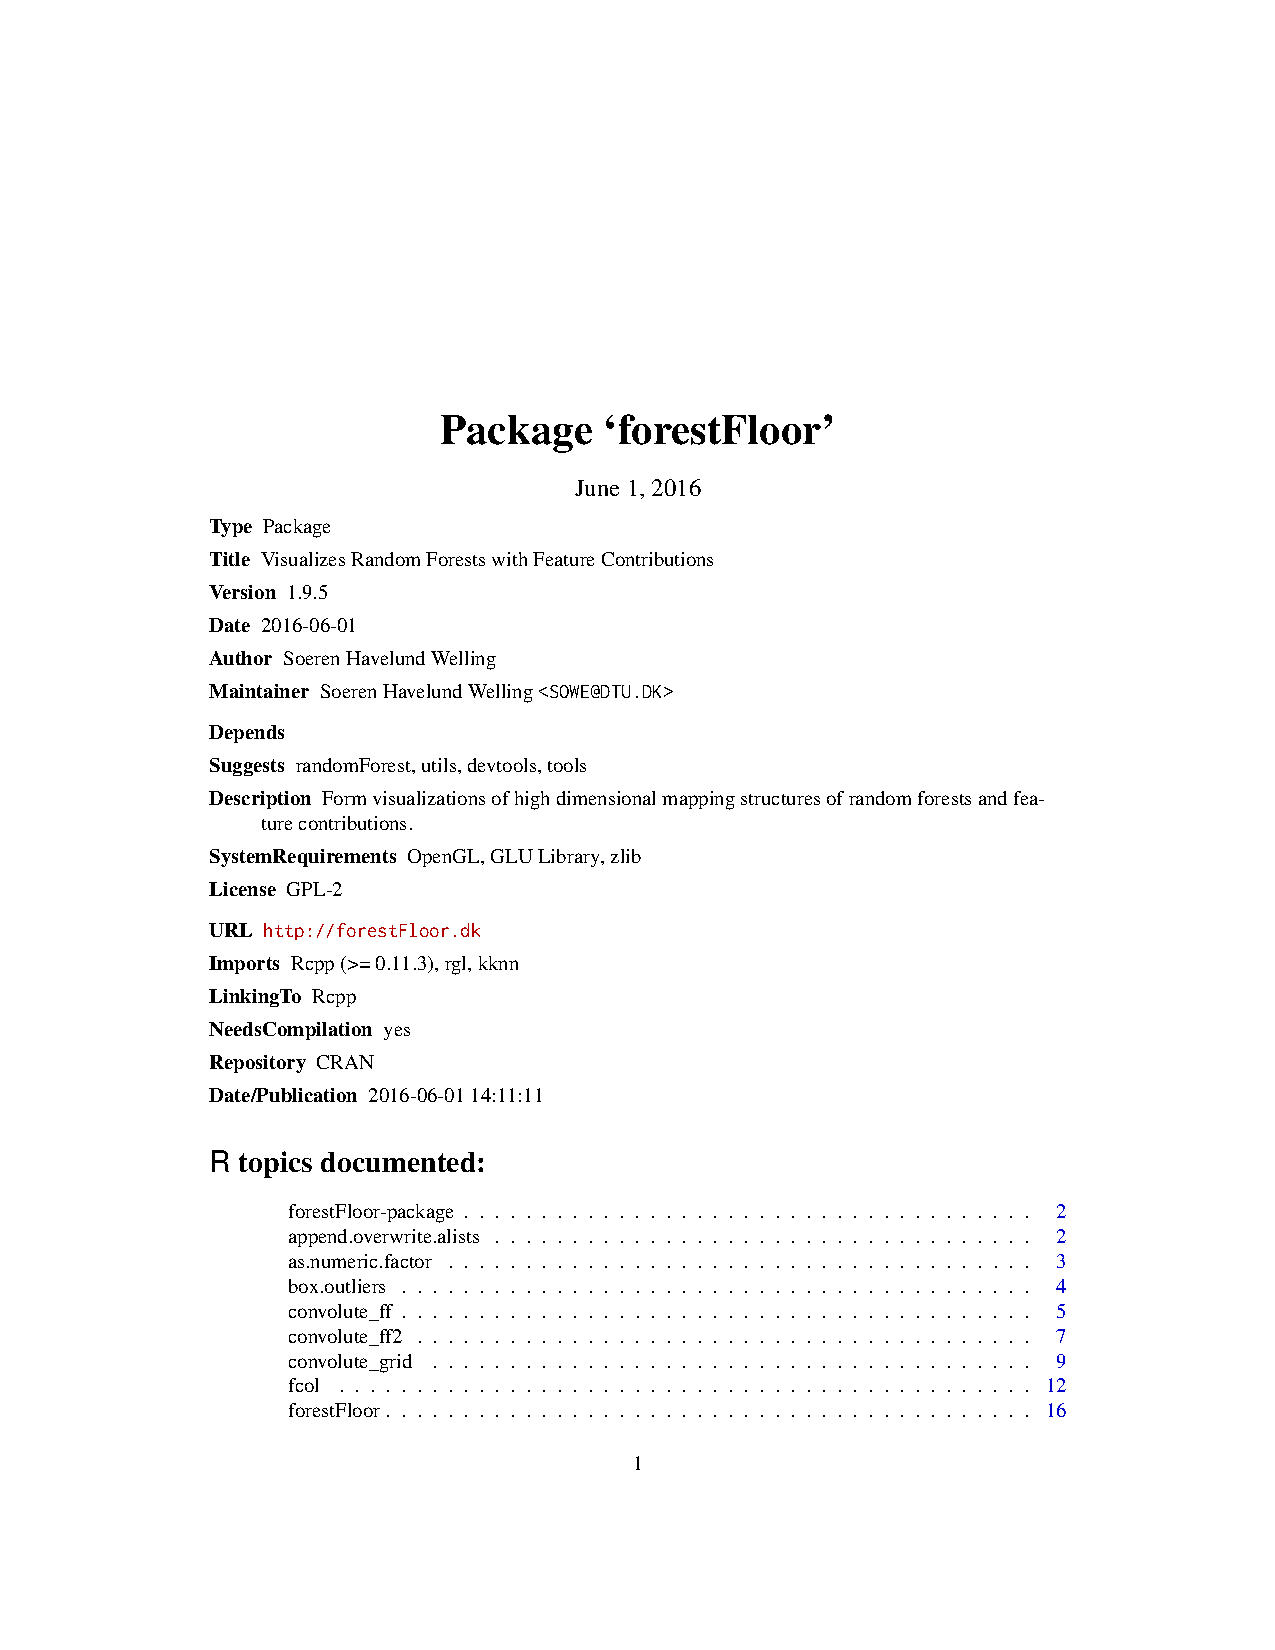
\includepdf[pages={1-},scale=0.90,pagecommand={\pagestyle{myruled}}]{appendices/forestFloorManual.pdf}

